\documentclass{article}
\usepackage{style-notes}

\newcounter{lecnum} 	% define counter for lecture number
\renewcommand{\thepage}{\thelecnum-\arabic{page}}	% define how page number is displayed (< lecture number > - < page number >)

% define lecture header and page numbers
% NOTE: to call use \lecture{< Lecture # >, < Lecture name >, < Chapter # >, < Chapter name >, < Section #s >}
\newcommand{\lecture}[5]{

    % define headers for first page
    \thispagestyle{empty} % removes page number from page where call is made

    \setcounter{lecnum}{#1}		% set lecture counter to argument specified

    % define header box
    \begin{center}
    \framebox{
      \vbox{\vspace{2mm}
    \hbox to 6.28in {\textbf{MATH 320: Probability} \hfill}
       \vspace{4mm}
       \hbox to 6.28in {{\hfill \Large{Lecture #1: #2} \hfill}}
       \vspace{2mm}
       \hbox to 6.28in {\hfill Chapter #3: #4 \small{(#5)}}
      \vspace{2mm}}
    }
    \end{center}
    \vspace{4mm}
    
    % define headers for subsequent pages
    \fancyhead[LE]{\textit{#2} \hfill \thepage} 		% set left header for even pages
    \fancyhead[RO]{\hfill \thepage}		% set right header for odd pages

}

% define macros (/shortcuts)
\newcommand{\bu}[1]{\textbf{\ul{#1}}}				% shortcut bold and underline text in one command
\newcommand{\blankul}[1]{\rule[-1.5mm]{#1}{0.15mm}}	% shortcut for blank underline, where the only option needed to specify is length (# and units (cm or mm, etc.)))
\newcommand{\vectwo}[2]{#1_1, \ldots, #1_{#2}}	% define vector (without parentheses, so when writing out in like a definition) of the form X_1, ..., X_k, where X and k are variable. NOTE: to call use $\vectwo{X}{k}$
\newcommand{\follow}[1]{\sim \text{#1}\,}		% shortcut for ~ 'Named dist ' in normal font with space before parameters would go
\newcommand{\followsp}[2]{\overset{#1}\sim \text{#2}\,}		% (followsp is short for 'follow special') shortcut that can be used for iid or ind ~ 'Named dist ' in normal font with space before parameters would go
\newcommand{\integral}[4]{\displaystyle \int_{#1}^{#2} #3 \,\mathrm{d} #4}		% shortcut for large integral with limits and appending formatted dx (variable x)
\newcommand{\e}{\mathrm{e}}		% shortcut for non-italic e in math mode
\newcommand{\gam}[1]{\Gamma(#1)}		% shortcut for gamma function (variable)
\newcommand{\chisq}{\raisebox{2pt}{$\chi^2$}}		% shortcut for chi-square distribution (better formatted chi letter in math mode with square added)
\newcommand{\Beta}[2]{B(#1, #2)}		% shortcut for beta function B(variable1, variable 2)



% NOTES on what didn't cover

%---- in general
% going to be lots........ (not going as in depth on some topics for sake of time
% pretty much all of the theory explanations in lecture 11-1 (except the intro, covered that), 11-2 and 11-3. Strategy at some point should be to have a version typed up that I teach (similar to what actex goes through), and then additional topics that is written out for me mainly (where it goes over all of the intuition from Dr. Kim
% --- The version here is going to be an abbreviated actex because of timing, so just giving what is needed to solve problems and only blurbs about extra explanations
% Theory summary of how to model different populations using the functions of the distributions we learned (like if X ~ gamma and Y = -X to model negative left skewed dist) (end of lecture 11-2)

%---- Uniform
% Lazar 3.1 motivation of the uniform density function (from the cdf)
% actex 8.1.5 conditional probability problem involving the uniform distribution (going to make it a hw problem)

%---- Exponential
% Proof that exp is waiting time between poisson (actex 8.2.9) and beginning of prob and stat inference 3.2, lazar's 3.2 (remark 3.22)
% Actex 8.2.6 another look at the meaning of the density function (used in their proof of above bullet)
% Actex 8.2.7 failure (hazard) rate, prob and stat inference has a little blurb on page 98 (that kinda goes with their memoryless example)

%---- Gamma
% Proof that gamma is waiting time between poisson alpha poisson events (prob and stat inference page 98)
% alternate way to show gamma dist is a valid pdf, change of variable to calculus way (lazar 3.2 in the definition of the pdf)
% Theory motivation behind gamma pdf pieces and their impact (lecture 11-2)
% Alternate way to calculate gamma probabilities (with Poisson) (in book and lazar notes maybe, and ask drew notes)

%---- Normal
% (Theory lecture 11) Three reasons why the normal distribution plays a central role
% (Theory lecture 11) Explanation of how came up with the density function (playing with e^-x)
% Continuity correction (Actex 8.4.6)
% Lazar empirical rule (3.3 notes)
% Combining two normal random variables (Lazar 3.3, last part of his 3.3 notes)
% textbook covers chi-square here, obviously not doing that now


\begin{document}

\lecture{11}{Continuous Distributions}{3}{Distributions}{3.1, 3.2, 3.3}

\bu{Introduction}\bigskip

\begin{itemize}
    \item Recall that statistical distributions are used to model populations; this is the goal!
    \item Suppose an insurance company has the following data from two samples of $n = 900$ policyholder losses for two different policies.
    \item[] We can think of these as observations from loss random variables $X$ and $Y$.
    \begin{figure}[H]
       \begin{minipage}{0.45\textwidth}
            \center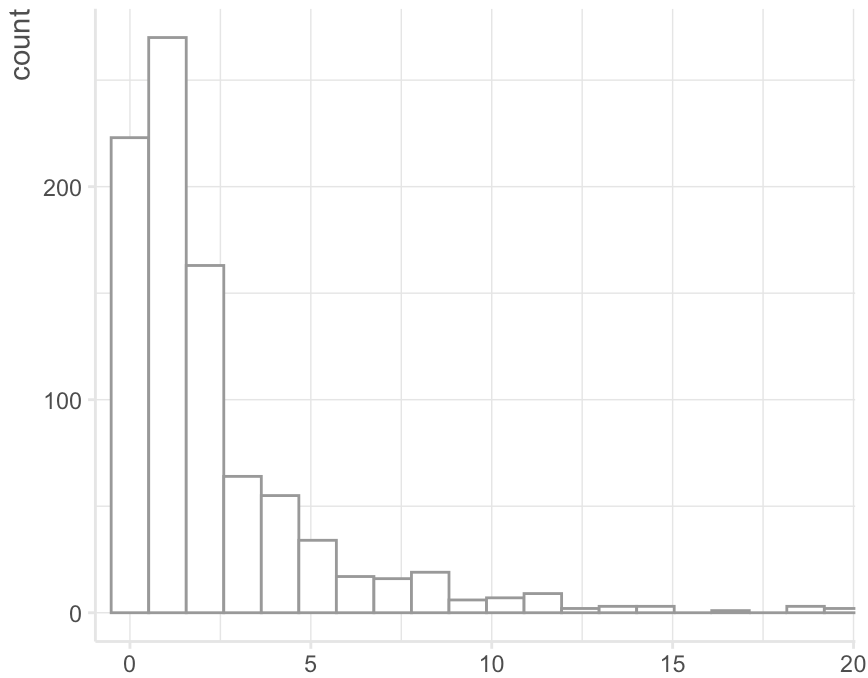
\includegraphics[scale=0.35]{test-3/hist-1}
        \end{minipage}
       \begin{minipage}{0.45\textwidth}
            \center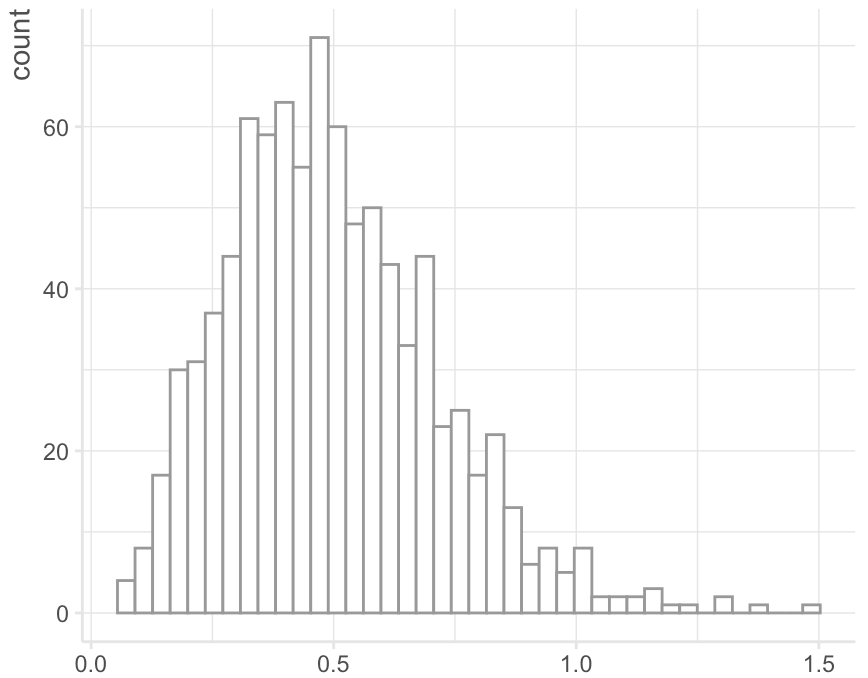
\includegraphics[scale=0.35]{test-3/hist-2}
        \end{minipage}
    \end{figure}
    \item The question is: How can me model the population that these losses are coming from?
    \item[] Said another way: In theory there is some distribution that these losses follow, and we want to figure out which family it is and what the parameter values are  $\Longrightarrow$ Find equation for smooth curve.
    \item Once the researcher knows this, they can figure out lots of things that are useful in analyzing how losses will occur in the future. For example (suppose $X$ is in thousands of dollars):
    \begin{itemize}
        \item Can find the expected claim amount $E(X)$. Then use this to set a premium amount to ensure at least breakeven.
        \item Can figure out the probability of ``major'' losses, say $P(X > 15 = \$15,000)$.
        \item Or if there is a deductible of say \$2,000, can find the percentage of claims that the insurance company is not responsible to pay for: $P(X < 2 = \$2,000)$.
    \end{itemize}\newpage
    \item If we already have data, we could simply approximate these values with empirical formulas:
    \begin{itemize}
        \item $\displaystyle E(X) \approx \frac{1}{n} \sum_{i = 1}^{n} x_i$\bigskip
        \item $P(X > 15 = \$15,000) \approx $\bigskip
        \item $P(X < 2 = \$2,000) \approx $\bigskip
    \end{itemize}
    \item But these are just approximations and are based on a single sample of data. Having population information is much better and much more generalizable!
    \item[] Observation: When we overlay these density curves, they match the histograms excellently.
    \begin{figure}[H]
       \begin{minipage}{0.45\textwidth}
            \center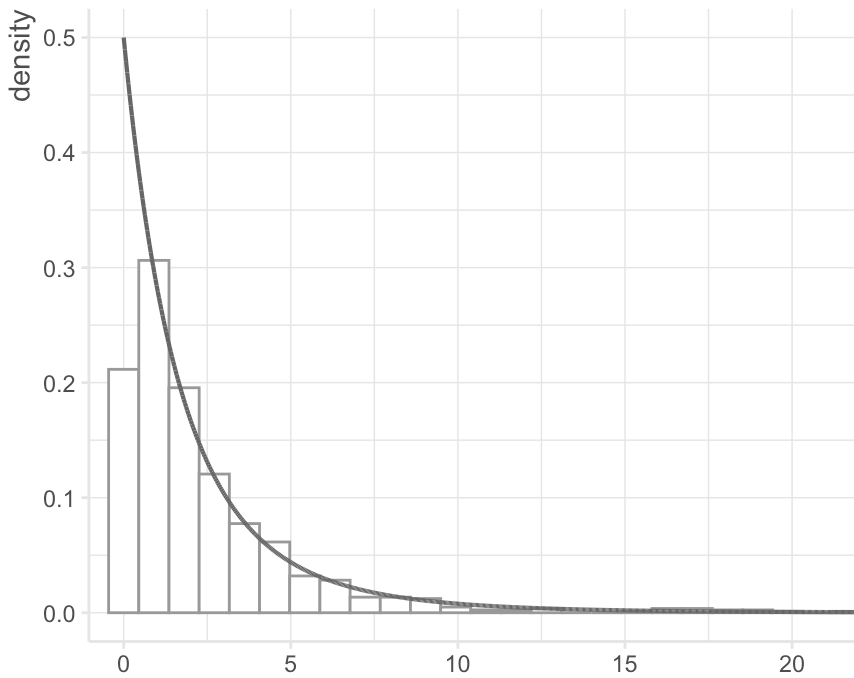
\includegraphics[scale=0.35]{test-3/hist-1-density}
        \end{minipage}
       \begin{minipage}{0.45\textwidth}
            \center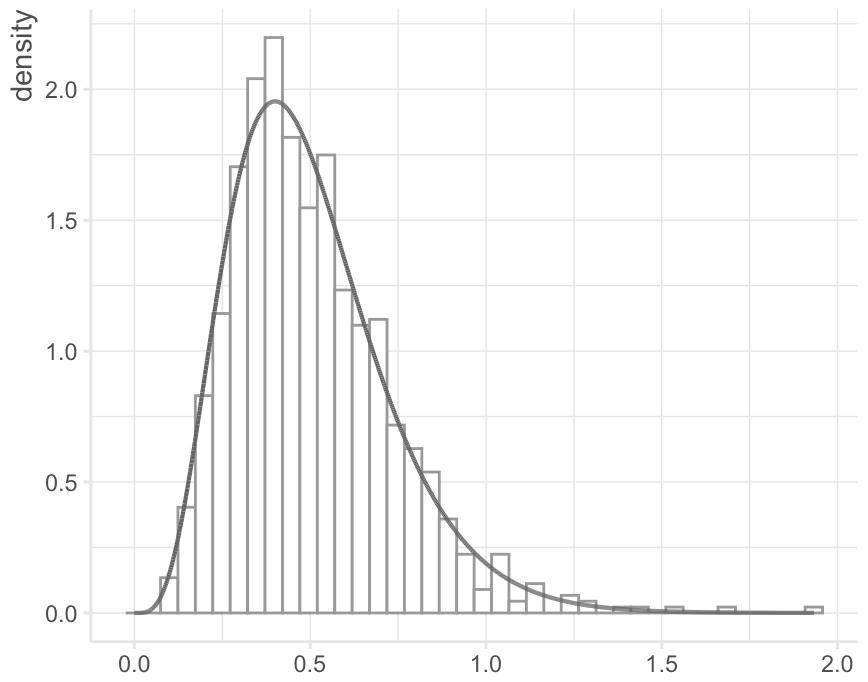
\includegraphics[scale=0.35]{test-3/hist-2-density}
        \end{minipage}
    \end{figure}
    \item Here is an overview of different population shapes and the distributions families that can be used to model them.
    \item If a population is distributed evenly between two numbers like
    \begin{figure}[H]
        \center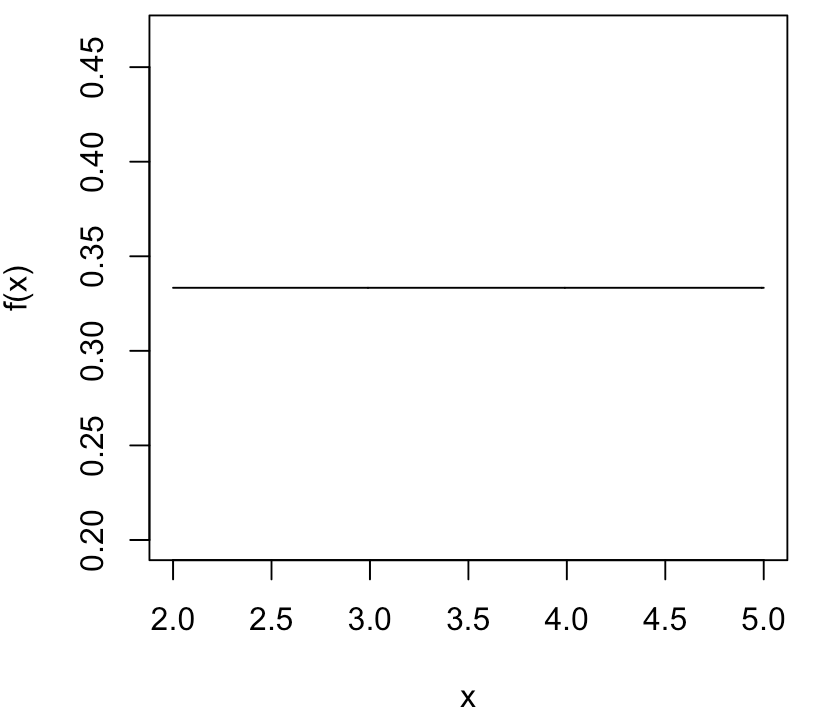
\includegraphics[scale=0.35]{test-3/uniform}
    \end{figure}
        \blankul{2cm} distribution must be used.\bigskip
    \item If a population is bell-shaped and symmetric like
    \begin{figure}[H]
        \center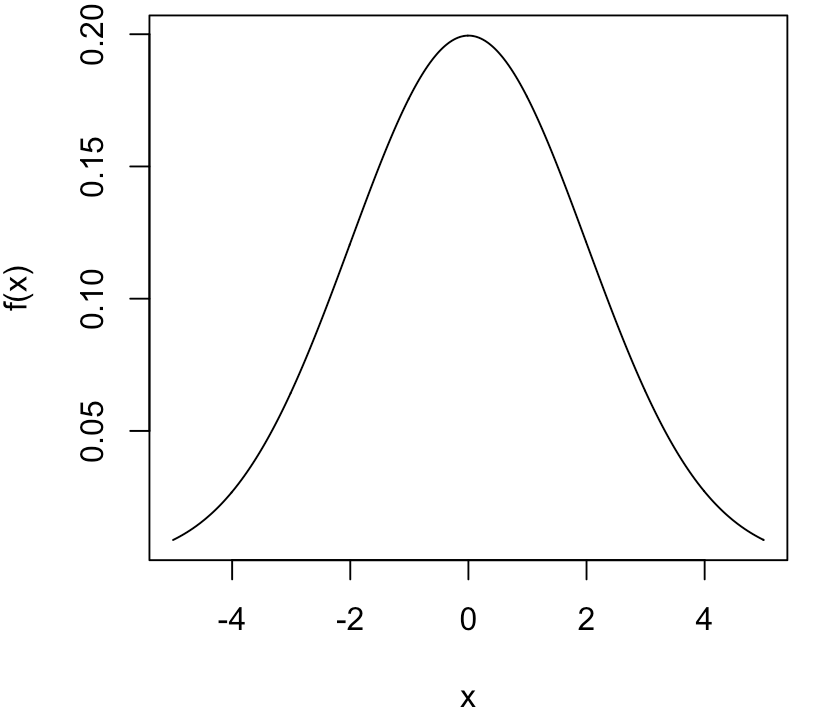
\includegraphics[scale=0.3]{test-3/bell-shaped}
    \end{figure}
        \blankul{2cm} or \blankul{2cm} distributions can be used, among others.\bigskip
    \item If a population is skewed like
    \begin{figure}[H]
        \center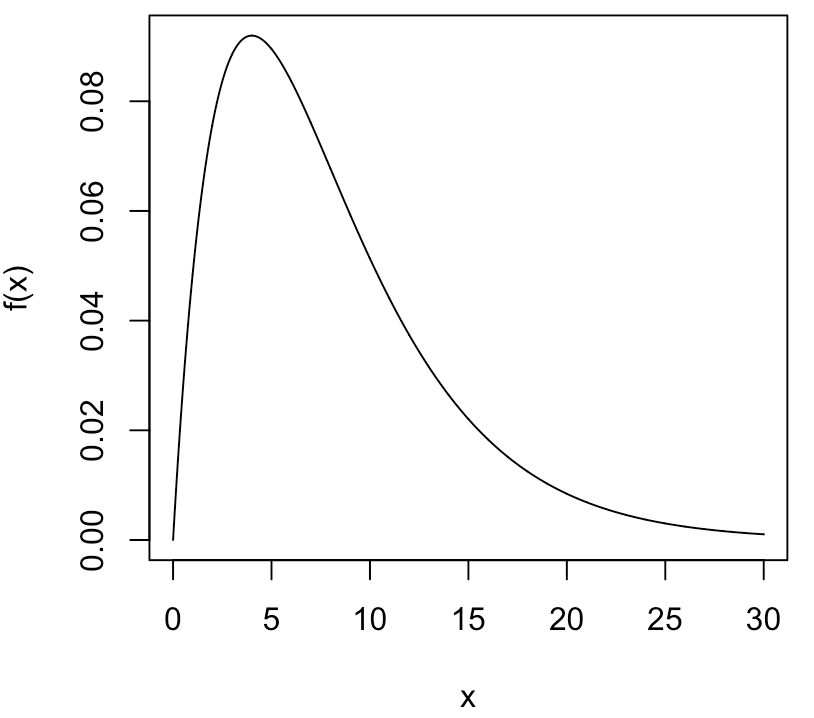
\includegraphics[scale=0.3]{test-3/skewed}
    \end{figure}
        \blankul{2cm}, \blankul{2cm} or \blankul{2cm} distributions can be used, among others.\bigskip
    \item If a population has bounded range (support) between two points and is not evenly distributed
    \begin{figure}[H]
        \center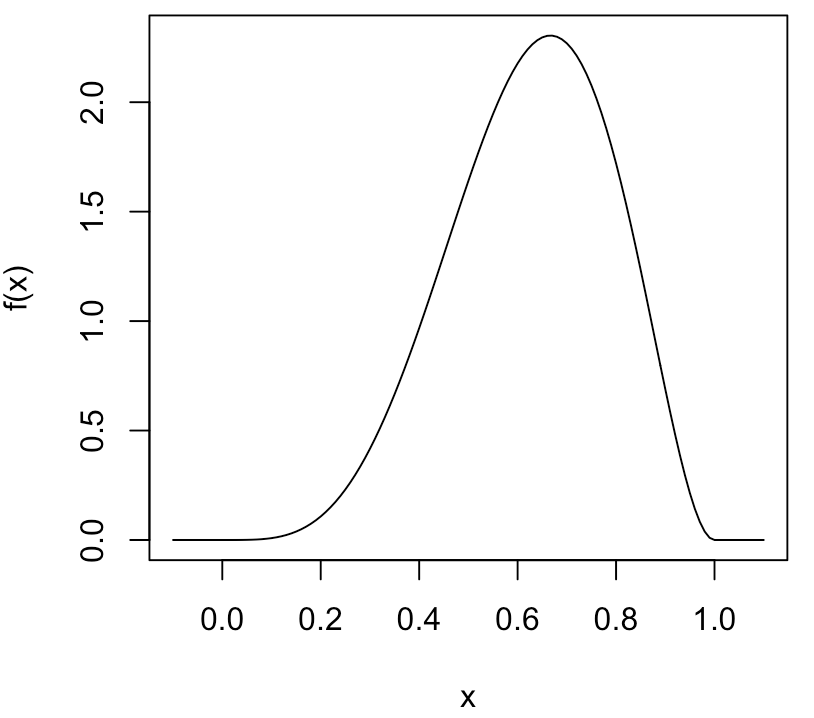
\includegraphics[scale=0.35]{test-3/non-symmetric-bounded}
    \end{figure}
        \blankul{2cm} distribution can be used. This is useful when modeling \blankul{3cm}.
\end{itemize}\bigskip

Very cool tangent!\bigskip
\begin{itemize}
    \item We saw in the previous example that we could model the data with a gamma distribution, specifically:
    \[Y \follow{Gamma}(\alpha = 5, \beta = 10)\]
    \item In practice, once the researcher selects the family (gamma), they would then have to estimate the parameter values using techniques such as maximum likelihood estimation (will learn this next semester!).
    \begin{itemize}
        \item The goal would be to have: $\hat{\alpha} \approx 5$ and $\hat{\beta} \approx 10$.
        \item This strategy would be in the context of Classical statistics, where parameter values are fixed constants; there is another branch of statistics called Bayesian statistics.
    \end{itemize}
    \item In Bayes, parameters are considered random variables and can have their own probability distributions. For example: $\alpha \follow{Exponential}(3)$ and $\beta \follow{Uniform}(1, 5)$.
\end{itemize}\bigskip

\bu{Uniform distribution}\bigskip

Definition\bigskip
\begin{itemize}
    \item The continuous uniform distribution is defined by spreading probability uniformly over an interval $[a,b]$ ($X$ can also be thought of as the outcome when a point is randomly selected from the interval $[a,b]$).
    \item If $X \follow{Uniform}(a, b)$
    \[
    f(x \mid a, b) =
        \left\{
        \begin{array}{ll}
            \displaystyle \frac{1}{b - a} & \quad a \le x \le b\\
            0 & \quad \text{otherwise}\\
        \end{array}
        \right.
    \]
    \item[] where the parameters $a$ and $b$ are real numbers.\bigskip
    \item Characteristics of a uniform distribution.
    \begin{itemize}
        \item Constant probability over the entire interval.
        \item Bounded support.
        \item Symmetric.
    \end{itemize}
\end{itemize}

\newpage

Probabilities\bigskip
\begin{itemize}
    \item The probability of any subinterval in the range (support) is proportional only to the \blankul{2cm} of the subinterval.\bigskip
    \item For $a \le c \le d \le b$
    \[P(c \le X \le d) = \]\bigskip
    \item We can generalize this to find $P(X \le x)$ for values of $x$ in the interval $[a,b]$.
    \item[] $P(X \le x) = $\vspace{20pt}
    \item Then we can define the cdf $F(x)$ for a uniform random variable $X$ on $[a,b]$ by:
    \[
    F(x \mid a, b) =
        \left\{
        \begin{array}{ll}
            0 & \quad\quad x < a\\\\
             & \quad\quad a \le x \le b\\\\
            1 & \quad\quad x > b\\
        \end{array}
        \right.
    \]
\end{itemize}\bigskip

Lifetime random variables and survival functions\bigskip
\begin{itemize}
    \item In many applied problems, the random variable interest is a time variable $T$. This time could represent:
    \begin{itemize}
        \item Time until death of a person (a standard insurance application).
        \item Time until the machine part fails.
        \item Time until a disease ends.
        \item Time it takes to serve a customer in a store.
    \end{itemize}
    \item The uniform distribution doesn't give a very realistic model of human lifetimes, but is often used as an illustration of a lifetime model because of its simplicity.
    \item Example: Let $T$ be the time from birth until death of a randomly selected member of a population. Assume that $T$ has a uniform distribution on $[0,100]$. Then
    \[
    f(t) =
        \left\{
        \begin{array}{ll}
            1/100 & \quad 0 \le t \le 1\\
            0 & \quad \text{otherwise}\\
        \end{array}
        \right.
    \hspace{20pt} \text{and} \hspace{20pt}
    F(t) =
        \left\{
        \begin{array}{ll}
            0 & \quad t <  0\\
            t/100 & \quad 0 \le t \le 1\\
            1 & \quad t > 100\\
        \end{array}
        \right.
    \]
    \begin{itemize}
        \item The function $F(t)$ gives us the probability that the person dies by age $t$.
        \item For example: The probability of death by age 57 is\bigskip
        \item Most of us are interested in the probability that we will survive past a certain age. In this example, we might wish to find the probability that we survive beyond age 57. This is simply the probability that we do \textit{not} die by age 57.\vspace{40pt}
    \end{itemize}
    \item The probability of surviving from birth past a given age $t$ is called a \textbf{survival probability} and denoted by $S(t)$.\bigskip
    \item Definition: The \textbf{survival function} is
    \[S(t) = P(T > t) = 1 - F(t)\]\vspace{20pt}
    \item The survival function for a uniform random variable is\vspace{80pt}
\end{itemize}\bigskip

Mean and variance\bigskip
\begin{itemize}
    \item If $X \follow{Uniform}(a, b)$\smallskip
    \[E(X) = \frac{a + b}{2} \hspace{80pt} V(X) = \frac{(b - a)^2}{12}\]
\end{itemize}\bigskip

Summarizing example\bigskip
\begin{itemize}
    \item Let $T$ be the time in months from initial use of a machine part until failure, where $T \follow{Uniform}(1, 9)$.
    \begin{enumerate}[a)]
        \item Find the pdf, cdf and survival function of $T$.\vspace{80pt}
        \item Find the probability the machine part fails between 5 and 7 months.\vspace{80pt}
        \item Find the probability the machine part lasts longer than 4 months.\vspace{80pt}
        \item Find the expected value and standard deviation for the lifetime of the machine part.\vspace{80pt}
    \end{enumerate}
\end{itemize}\bigskip

\bu{Exponential distribution}\bigskip

(Brief) Motivation\bigskip
\begin{itemize}
    \item Recall when observing a Poisson process, we counted the number of occurrences in a given interval. This number was a discrete random variable with a Poisson distribution.\vspace{40pt}
    \item But not only is the number of occurrences a random variable, the waiting times between successive occurrences are also random variables. These are continuous and follow an exponential distribution.
    \item Formal statement: It can be shown that the exponential distribution gives the probability for the waiting time between successive Poisson events.
\end{itemize}

\newpage

Derivation of density\bigskip
\begin{itemize}
    \item The main part of the density function is an exponential decay function with parameter $\lambda$, which represents average number of events occurring (i.e. average rate of events) per unit of time in a Poisson process.\smallskip
    \item To get this function to be a valid pdf, when integrated over the appropriate range $[0, \infty)$ it needs to equal 1.\vspace{130pt}
    \item[] This process is the same as finding $c$ such that: \vspace{20pt}
    \item The value $c$ is called a \textbf{normalizing constant}.
    \begin{itemize}
        \item All of the distributions we will study from now on have a normalizing constant, some of which are quite complex.
        \item The purpose is the same though, functions of $x$ determine the shape of a function (e.g. $\e^{-\lambda x}$), then $c$ converts it to a valid pdf.
    \end{itemize}
\end{itemize}\bigskip

Definition\bigskip
\begin{itemize}
    \item If $T \follow{Exponential}(\lambda)$
    \[f(t \mid \lambda) = \lambda \e^{-\lambda t}, \quad\quad t \ge 0 \quad \text{and}\quad \lambda > 0\]
    \item Characteristics of an exponential distribution.
    \begin{itemize}
        \item Gives the probability for the waiting time between successive Poisson events.
        \item Right-skewed density function.
        \item Unbounded support.
        \item The exponential random variable is a continuous version of the \blankul{3cm} random variable, which waits for the first \blankul{2cm} in a discrete sample space.
        \item Also has the \blankul{3cm} property: $P(T > a + b \mid T > a) = P(T > b)$.
        \item[] Exponential and geometric are the only distributions with the memoryless property.
    \end{itemize}
\end{itemize}\bigskip

Parameter\bigskip
\begin{itemize}
    \item As stated, $\lambda$ is the rate at which events occur in a Poisson process. Here is how it affects the exponential density function.
    \item As $\lambda$ increases, events happen more often in a time interval, which consequently means we are waiting less and less for the next event to occur.
    \begin{figure}[H]
        \center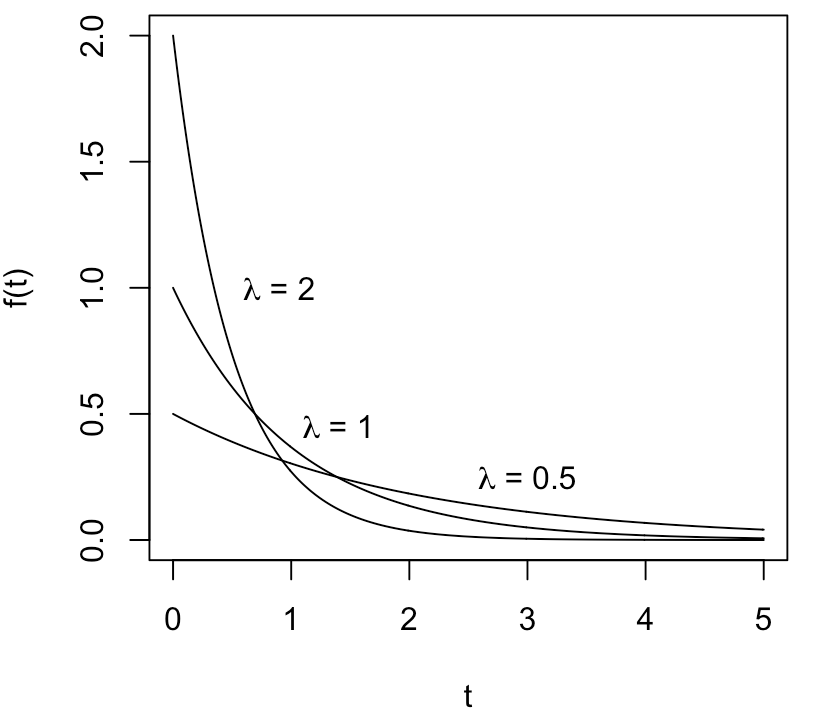
\includegraphics[scale=0.45]{test-3/exp}
    \end{figure}
    \item[] We see that for larger values of $\lambda$, there is more probability close to zero and less in the tail.
    \item Just like with some of the discrete distributions, there are different versions of the exponential distribution.
    \begin{itemize}
        \item All versions have a random variable that is giving probabilities for waiting times. So they are not different in the way that we had two different versions of the geometric random variable (counting number of trials vs number of failures).
        \item Rather they differ in what the parameters represent.
        \begin{enumerate}
            \item The definition given above uses the \textbf{rate parameterization} of the exponential distribution.
            \item There is also a \textbf{scale parameterization}, where the scale parameter $\theta$ is defined by
            \item[] $\displaystyle \text{scale } \theta = \frac{1}{\text{rate}} = \frac{1}{\lambda} \hspace{20pt}\Longrightarrow \hspace{20pt}$
        \end{enumerate}
        \item This obviously will impact the formulas for the cdf, mean, variance, etc.
    \end{itemize}
\end{itemize}

\newpage

Probabilities\bigskip
\begin{itemize}
    \item Probabilities for the exponential distribution are easy to solve by hand (unlike the next distributions).
    \item Example: Accidents at a busy intersection occur at an average rate of $\lambda = 2$ per month according to a Poisson process. Let $T$ be the random variable for the time between accidents.
    \begin{enumerate}[a)]
        \item Find $f(t)$.\vspace{20pt}
        \item Cdf $P(T \le t)$: Find the probability that the waiting time for the next accident is less than 2.\vspace{70pt}
        \item Survival $P(T > t)$: Find the probability that the waiting time for the next accident is longer than 1 month.\vspace{70pt}
        \item Interval $P(a \le X \le b)$: Find the probability that the waiting time for the next accident is between 0.5 and 1.5 months\vspace{100pt}
    \end{enumerate}
    \item Cdf and survival function:
    \item[] If $T \follow{Exponential}(\lambda)$
    \[F(t) =  \hspace{150pt} S(t) = \]\vspace{20pt}
    \item[] Note that we could derive these formally:
    \item Using the cdf: Recall once the cdf $F(x)$ is known for a random variable $X$, it can be used to find the probability that $X$ lies in any interval since
    \[P(a \le X \le b) = \]
    \item[] For the exponential distribution, we have:\bigskip
    \item[] $P(a \le T \le b) = $
\end{itemize}\bigskip

Mean and variance\bigskip
\begin{itemize}
    \item If $T \follow{Exponential}(\lambda)$\smallskip
    \[E(T) = \frac{1}{\lambda} \hspace{80pt} V(T) = \frac{1}{\lambda^2}\]\bigskip
    \item Example: Find the mean and variance for the previous accident example:\bigskip
\end{itemize}\bigskip

Memoryless property\bigskip
\begin{itemize}
    \item Just like the geometric distribution, the exponential distribution has the \textbf{memoryless property}.
    \item Theorem: If $T \follow{Exponential}(\lambda)$
    \[P(T > a + b \mid T > a) = P(T > b)\]
    \item (Using a concrete example to help conceptualize) The probability that a bulb will operate for more than time $a + b$ time units, given that has already operated for at least $a$ time units, is the same as the probability that a new bulb will operate for at least $b$ time units.
    \item[] In practical terms, this means that the length of time a light bulb has already operated does not affect its chances of operating for additional time units.
    \begin{figure}[H]
        \center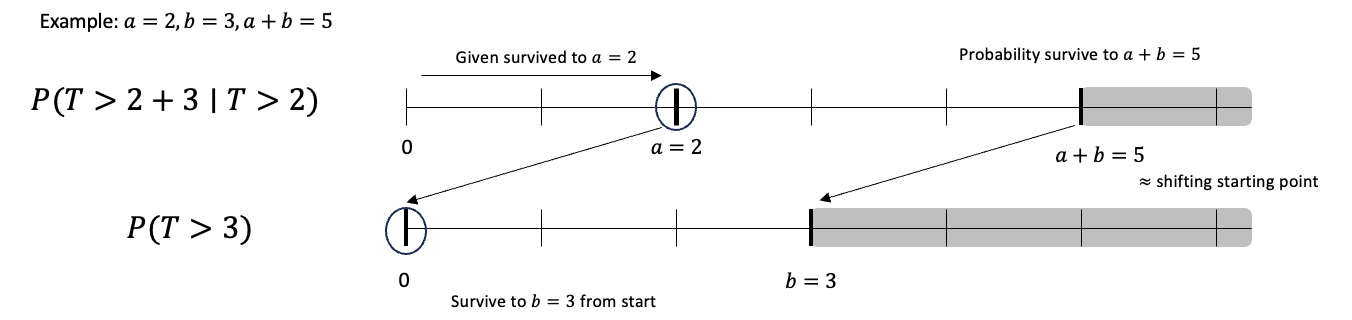
\includegraphics[scale=0.6]{test-3/memoryless}
    \end{figure}
    \item Proof:\vspace{60pt}
    \item Example: Let $T$ be the time to failure of a machine part, where \\ $T \follow{Exponential}(\lambda = 0.001)$.
    \begin{enumerate}[(a)]
        \item Given that the part has operated 100 hours, find the probability it will operate for 150 hours.\vspace{40pt}
        \item Given that the part has operated 100 hours, find the probability it will operate for $100 + x$ hours ($0 \le x < \infty$).\vspace{40pt}
    \end{enumerate}
    \item Note that survival functions are unique, just like cdfs and pdfs.
    \item[] And the final expression in part (b) is the survival function $S(x)$ for a random variable which is exponentially distributed on $[0, \infty)$ with $\lambda = 0.001$; so it must have this distribution. This has a nice intuitive interpretation:
    \begin{itemize}
        \item Lifetime of a new part $\sim$
        \item Remaining lifetime of a 100 hr old part $\sim$
    \end{itemize}
\end{itemize}\bigskip

Waiting time for a Poisson process\bigskip
\begin{itemize}
    \item In the intro, we stated that the exponential distribution gives the waiting time between Poisson events. Here's why.
    \item If the number of events in a time period of length 1 is a Poisson random variable with parameter $\lambda$, then the number of events in a time period of length $t$ is a Poisson random variable with parameter \blankul{1cm}. Let this be the random variable $X$.
    \item[] This is a reasonable assumption (think about the accidents in 1 month vs 3 months example).
    \item We can find the probability of no accidents in an interval of length $t$ easily:\vspace{30pt}
    \item[] However, no accidents in an interval of length $t$ is equivalent to saying the waiting time $T$ for the next accident is greater than $t$. Thus\vspace{30pt}
    \item Example: Customers arrive in a certain shop according to an approximate Poisson process at a mean rate of 40 per 2 hours. What is the probability that the shopkeeper will have to wait more than 5 minutes for the arrival of the first customer?\vspace{80pt}
\end{itemize}\bigskip

Last example\bigskip
\begin{itemize}
    \item The lifetime of a machine has an exponential distribution with a mean of 3 years. The manufacturer is considering offering a warranty and considers two types of warranties.
    \begin{itemize}
        \item Warranty 1 pays 3 if the machine fails in the first year, 2 if the machine fails in the second year, and 1 if the machine fails in the third year, with no payment if the machine fails after 3 years.
        \item Warranty 2 pays $3\e^{-T}$ at time $T$ years.
    \end{itemize}
    \item[] Find the expected warranty payment under each of the two warranties.\vspace{150pt}
\end{itemize}

\newpage

\bu{Gamma distribution}\bigskip

(Brief) Motivation\bigskip
\begin{itemize}
    \item Relationship between the exponential distribution and the gamma distribution:\vspace{200pt}
    \item The gamma distribution can also applied in other problems where the exponential distribution is useful like analysis of failure time of a machine part or survival time for a disease.
\end{itemize}\bigskip

Definition\bigskip
\begin{itemize}
    \item If $X \follow{Gamma}(\alpha, \beta)$
    \[f(x \mid \alpha, \beta) = \frac{\beta^\alpha}{\gam{\alpha}} \, x^{\alpha - 1} \, \e^{-\beta x}, \quad\quad x \ge 0 \quad \text{and}\quad \alpha, \beta > 0\]\vspace{20pt}
    \item Intuitive idea behind pdf: 
    \begin{itemize}
        \item The main part of $f(x)$ is $x^{\alpha - 1} \, \e^{-\beta x}$.
        \item[] As $x \rightarrow \infty , \, x^{\alpha - 1} \rightarrow \hspace{15pt}$ for $\alpha > 1$.
        \item[] As $x \rightarrow \infty , \, e^{-\beta x} \rightarrow \hspace{15pt}$ for $\beta > 0$.
        \item[] When $x$ is small, $x^{\alpha - 1} \, e^{-\beta x}$ is dominated by \blankul{2cm}; when $x$ is large, it is dominated by \blankul{2cm}. Thus as $x \rightarrow \infty , \, x^{\alpha - 1} \, e^{-\beta x} \rightarrow \hspace{15pt}$.
        
        \newpage
        
        \item Once we model the shape of the density function, we need to find the constant $c$ such that
        \[\integral{0}{\infty}{c \, x^{\alpha - 1} \, e^{-\beta x}}{x} = 1\]
        \item[] By some calculus, we can show that $c = \frac{\beta^\alpha}{\gam{\alpha}}$, where \[\gam{\alpha} = \integral{0}{\infty}{x^{\alpha - 1}\, \e^{-x}}{x}, \quad\quad \alpha > 0\]
    \end{itemize}
    \item The quantity $\gam{\alpha}$ is known as the \textbf{gamma function}. Here is a summary of the $\gam{\alpha}$:
    \begin{itemize}
        \item Gives a value for any $\alpha > 0$. 
        \item We can think of the gamma function as an extension of the factorial definition from the positive integers to all positive real numbers.
        \item[] Integration by parts can show
        \[\gam{t} = (t - 1) \, \gam{t - 1}\]
        \item Whenever $\alpha = n$, where $n$ is a positive integer, repeated integration by parts shows that
        \[\gam{n} = (n - 1) \, \gam{n - 1} = (n - 1) (n - 2) \cdots (2) (1) \, \gam{1}\]
        \vspace{30pt}
        \item[] Thus, when $n$ is a positive integer, we have
        \[\gam{n} = (n - 1)!, \quad\quad n = 1, 2, \ldots\]
        \item The pdf for the gamma distribution is essentially the gamma function as defined above, except it introduces another parameter in the exponential term, $\beta$.\bigskip
    \end{itemize}
    \item Characteristics of a gamma distribution:
    \begin{itemize}
        \item Gives the probability for the waiting time until the $\alpha^{th}$ occurrence in a  Poisson process.
        \item Right-skewed density function.
        \item Unbounded support.
        
        \newpage
        
        \item Two important special cases of the gamma distribution:
        \begin{enumerate}
            \item When $\alpha = 1 \rightarrow X \follow{Exponential}(\beta)$. Thus gamma can be considered a generalized version of the exponential random variable.\vspace{40pt}
            \item When $\alpha = r / 2, \;\; \beta = 2 \rightarrow X \follow{\chisq}(r)$ (read ``Chi-squared''). This distribution is important in statistical inference, especially in analysis of variance (aka ANOVA), which is the basis of experimental design methods.
        \end{enumerate}
    \end{itemize}
\end{itemize}\bigskip

Parameters\bigskip
\begin{itemize}
    \item The parameters of the distributions we have studied so far have a direct interpretation, but here $\alpha$ and $\beta$ do not. But we can still give some meaning to them. Here is how they affect the gamma density function.
    \item $\alpha = $ \textbf{shape} parameter.
    \begin{figure}[H]
        \center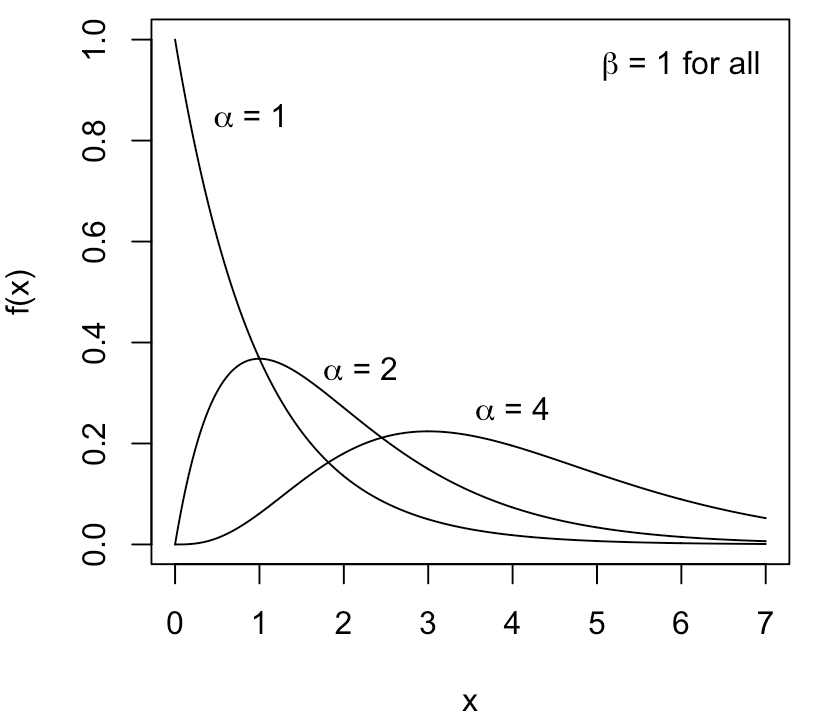
\includegraphics[scale=0.4]{test-3/gamma-shapes}
    \end{figure}
    \item[] We see that for different values of $\alpha$ (and constant $\beta$), there are different \blankul{1.5cm} of the gamma densities. Hence ``shape'' parameter.
    \item[] Additionally, for larger values of $\alpha$, the density increases longer out from zero because the polynomial part of the density function is more powerful for small $x$. 
    \item[] Notice that when \blankul{1cm} we have the familiar negative exponential curve. All exponential densities have this shape because of this fixed $\alpha$.
    
    \newpage
    
    \item $\beta = $ \textbf{rate} parameter (or $\theta = 1 / \beta = $ \textbf{scale} parameter).
    \begin{figure}[H]
        \center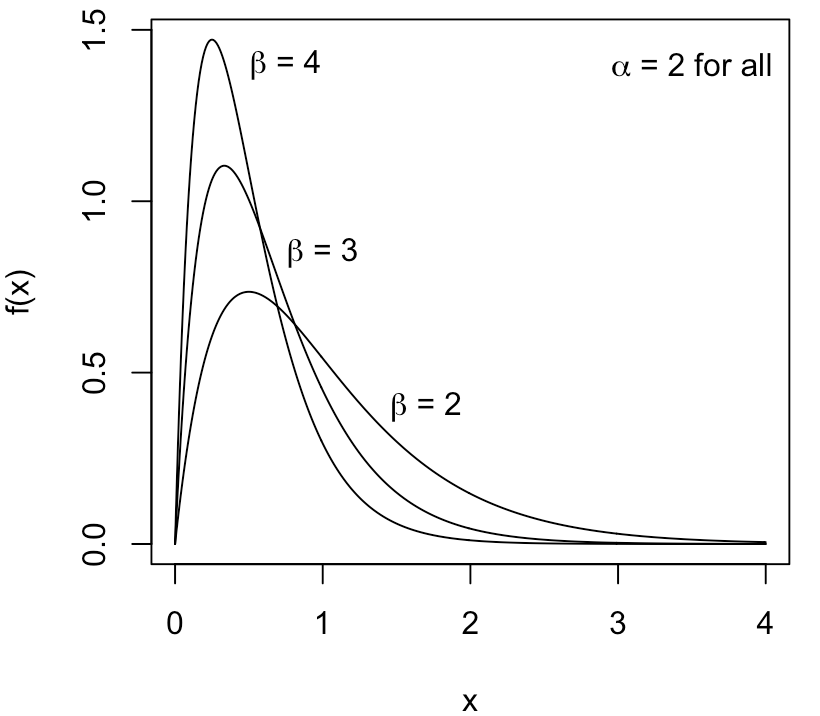
\includegraphics[scale=0.35]{test-3/gamma-scales}
    \end{figure}
    \item[] We see that for different values of $\beta$ and constant $\alpha$, the general \blankul{1.5cm} of the gamma densities look similar, but the \blankul{1.5cm} are different. Hence ``scale'' parameter, which is equal to the inverse rate.
    \item Remember that the rate vs scale parameterizations will cause slight differences in the formulas for the pdf, mean, variance, etc. in other resources.
\end{itemize}\bigskip

Probabilities\bigskip
\begin{itemize}
    \item Probabilities for the gamma distribution are difficult. If $X \follow{Gamma}(\alpha, \beta)$:
    \begin{itemize}
        \item Can only be solved by hand if $\alpha$ is an integer.
        \item[] $\alpha = 1 \rightarrow$ Exponential.
        \item[] $\alpha = 2 \rightarrow$ Requires integration by parts once.
        \item[] $\alpha > 2 \rightarrow$ Requires repeated integration by parts $\alpha - 1$ times.
        \item If $\alpha$ is not an integer and $0 < c < d < \infty$, we cannot calculate $P(c < X < d)$ by integration because it is impossible to give a closed-form expression for
        \[\integral{c}{d}{\frac{\beta^\alpha}{\gam{\alpha}} \, x^{\alpha - 1} \, \e^{-\beta x}}{x}\]
        \item[] Thus we must use statistical software to compute the probability that a gamma random variable falls in an interval.
        \item Software do implement a general gamma cdf, but not anything one needs to know.
    \end{itemize}
\end{itemize}\bigskip

Mean and variance\bigskip
\begin{itemize}
    \item If $X \follow{Gamma}(\alpha, \beta) \quad\quad \alpha, \beta > 0$\smallskip
    \[E(X) = \frac{\alpha}{\beta} \hspace{80pt} V(X) = \frac{\alpha}{\beta^2}\]
    \item If $\alpha = 1$, $E(X)$ and $V(X)$ for exponential follow.
\end{itemize}

\newpage

Summarizing examples:
\begin{enumerate}
    \item Let $X$ be random variable for the waiting time (in months) from the start of observation until the second accident at an intersection. Assume $X \follow{Gamma}(\alpha = 2, \beta = 3)$.
    \begin{enumerate}
        \item Find the pdf of $X$.\vspace{60pt}
        \item Find $E(X)$ and $V(X)$.\vspace{40pt}
        \item Find the probability the total waiting time for the second accident is between 1 and 2 months.\vspace{300pt}
    \end{enumerate}
    \item Biologists investigating a stretch of desert find certain fossils according to a Poisson process at a mean rate of 500 per kilometer.
    \item[] What is the probability that the biologists will have to investigate more than 5 meters in order to find the first four fossils?\vspace{50pt}
\end{enumerate}

\bu{Normal distribution}\bigskip

Applications\bigskip
\begin{itemize}
    \item The \textbf{normal distribution} is the most widely-used of all the distributions we have and will discuss. It can be used to model a wide range of natural phenomena that follow the ``bell-shaped'' pattern in their relative frequency distribution (histogram).
    \begin{figure}[H]
       \begin{minipage}{0.45\textwidth}
            \center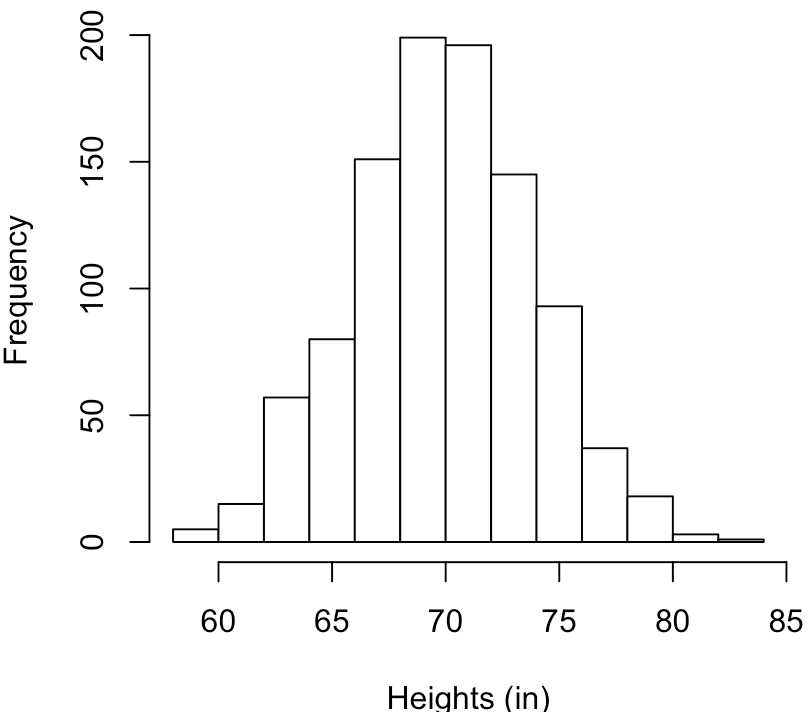
\includegraphics[scale=0.22]{test-3/normal-hist}
        \end{minipage}
       \begin{minipage}{0.45\textwidth}
            \center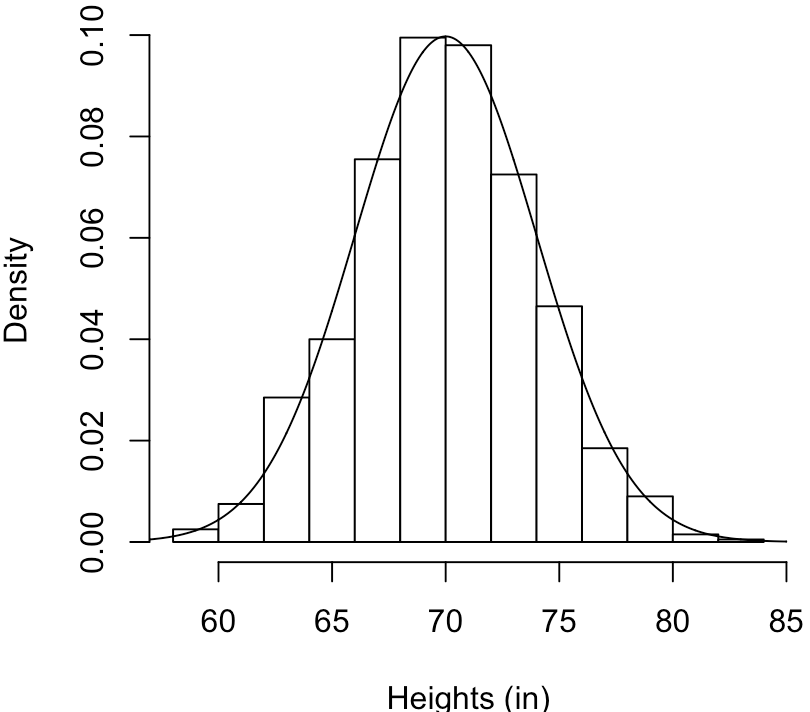
\includegraphics[scale=0.2]{test-3/normal-hist-density}
        \end{minipage}
    \end{figure}
    \item Examples include variables such as test scores, physical measurements (height, weight, length) of organisms, and repeated measurements of the same quantity on different occasions or by different observers (measurement error), stock portfolio returns, insurance portfolio losses, etc.
    \item Every normal density curve has this shape, and the normal density model is used to find probabilities for all of the natural phenomena who histograms display this pattern.
    \item Random variables whose histograms are well-approximated by a normal density curve are called \textbf{approximately normal}.
\end{itemize}\bigskip

Definition\bigskip
\begin{itemize}
    \item If $X \follow{Normal}(\mu, \sigma^2)$
    \[f(x \mid \mu, \sigma^2) = \frac{1}{\sqrt{2 \pi \sigma^2}} \, \exp\bigg[-\frac{(x - \mu)^2}{2\sigma^2}\bigg], \quad\quad -\infty < x < \infty \quad \text{and}\quad -\infty < \mu < \infty, \quad \sigma > 0\]\vspace{30pt}
    \item Intuitive idea behind pdf:
    \begin{enumerate}
        \item Set the shape $\rightarrow$ Bell-shaped and symmetric (exponential decay from center in both directions)
        \item Change to smooth curve
        \item Find constant to make valid pdf.
        \item Add location and scale parameters to shift and scale the density, respectively.
        \item Adjust constant to take into account new parameters.
    \end{enumerate}
    \item Characteristics of a normal distribution.
    \begin{itemize}
        \item Density function is bell-shaped and symmetric.
        \item Unbounded support (range).
        \item[] But the density decreases exponentially as $x$ runs away from the center. Thus, the normal distribution is also used for bounded data in practice (e.g. test scores).
    \end{itemize}\smallskip
    \item The density function for the normal distribution is difficult to integrate as we will see. For example, to show that the normal distribution is a valid pdf, we need to use polar coordinates.
\end{itemize}\bigskip

Parameters, expected value and variance\bigskip
\begin{itemize}
    \item The normal distribution is somewhat special in the sense that it's two parameters provide us with complete information about the exact shape (the spread) and location (where it's centered) of the distribution.
    \item If $X \follow{Normal}(\mu, \sigma^2)$
    \[E(X) = \mu \hspace{80pt} V(X) = \sigma^2 \hspace{80pt} SD(X) = \sigma\]
    \item These are really easy to derive using moment generating functions (will learn later).
    \item Here is how they affect the normal density function.
    \begin{figure}[H]
       \begin{minipage}{0.45\textwidth}
            \center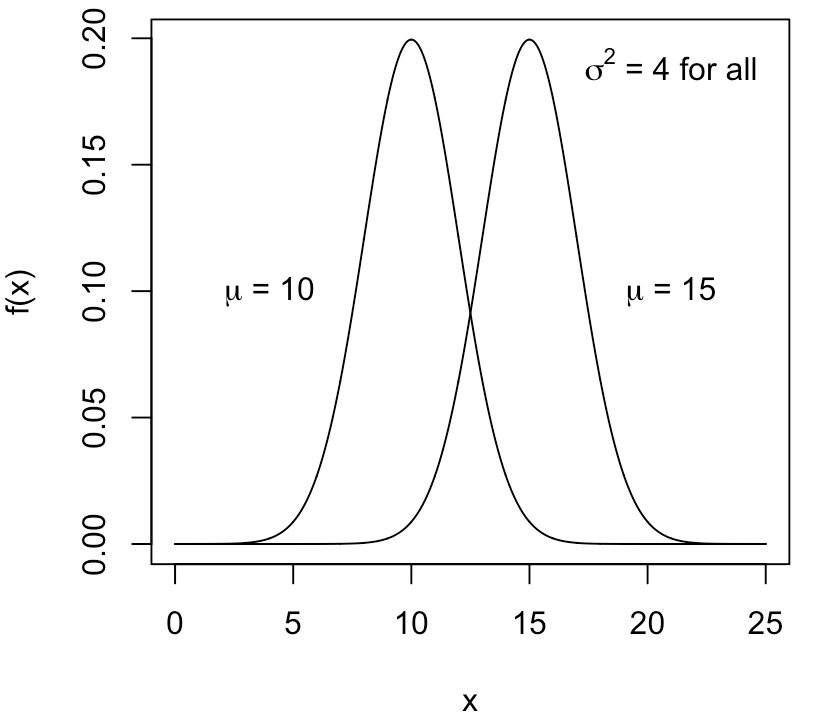
\includegraphics[scale=0.25]{test-3/normal-means}
        \end{minipage}
       \begin{minipage}{0.45\textwidth}
            \center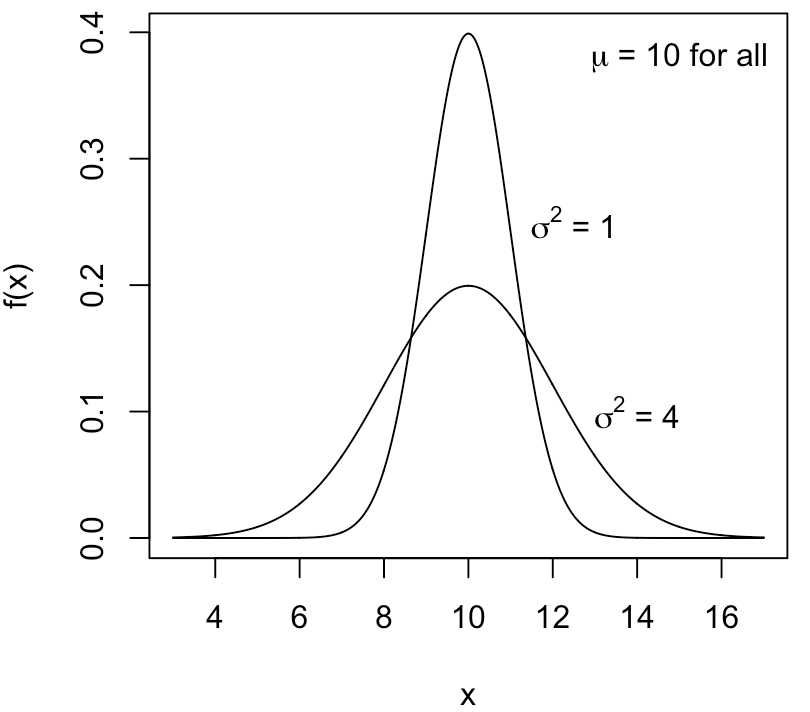
\includegraphics[scale=0.25]{test-3/normal-sds}
        \end{minipage}
    \end{figure}
    \item In practice, often the standard deviation $\sigma$ is used rather than the variance $\sigma^2$. So it is common to see $X \follow{Normal}(\mu, \sigma)$.
\end{itemize}\bigskip

Probabilities\bigskip
\begin{itemize}
    \item Suppose we are looking at a national exam whose scores $X$ are approximately normal with $\mu = 500$ and $\sigma = 100$. To find the probability a score is between 600 and 750, we have to evaluate the integral:\vspace{40pt}
    \item This cannot be done in closed-form (just like the gamma distribution), but it can be approximated using numerical methods using software, such as TI-84s as shown next.
    
    \newpage 
    
    \begin{figure}[H]
        \center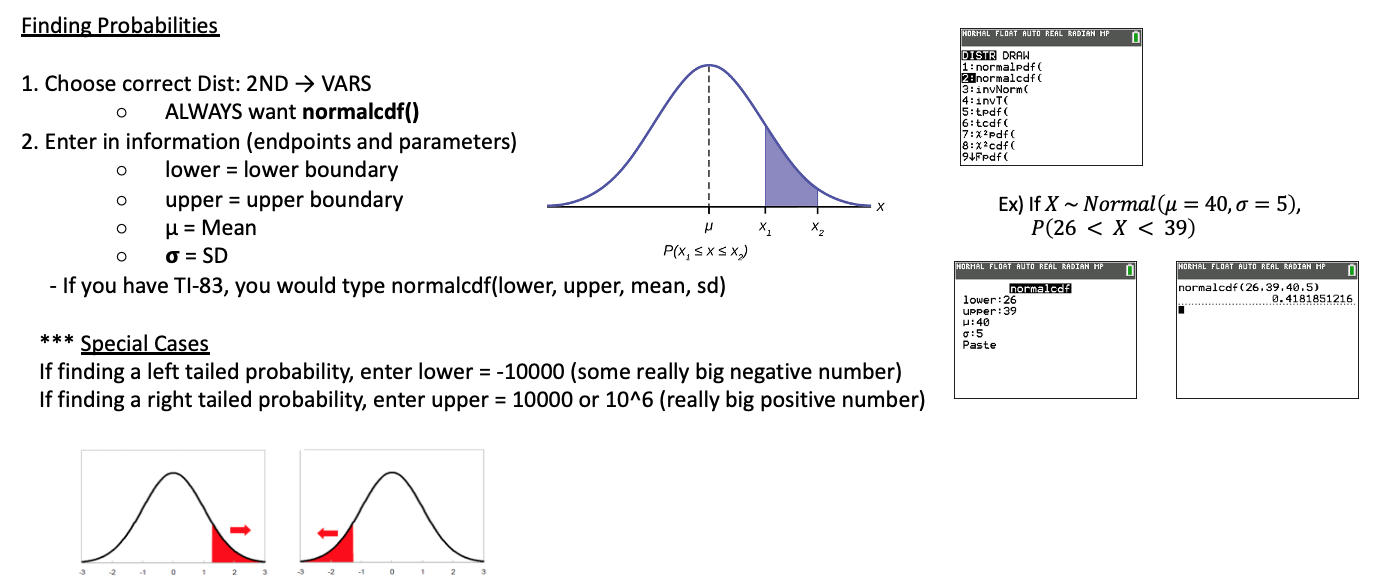
\includegraphics[scale=0.65]{test-3/normalcdf}
    \end{figure}
    \item In the olden days before such software was readily available, another way of finding normal probabilities involving tables of areas for a standard normal distribution was developed.
    \item[] \textit{NOTE}: Exam P formula sheet only gives LEFT probabilities for POSITIVE $Z$ values  $\Longrightarrow$ We need to use properties of the normal curve to find probabilities for $-Z$. So you have to know this way.
    \begin{figure}[H]
        \center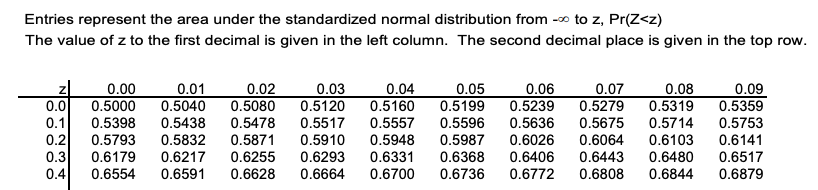
\includegraphics[scale=0.85]{test-3/z-table}
    \end{figure}\vspace{100pt}
    \item We will now cover this method, and the basic properties of the normal distribution which are behind it, in a series of steps.
    
    \newpage
    
    \item \textbf{Step 1: Linear transformation of normal random variables}\bigskip
    \begin{itemize}
        \item Theorem: If $X \follow{Normal}(\mu, \sigma^2)$ and $Y = aX + b$. Then
        \[Y \follow{Normal}(a\mu + b, a^2\sigma^2)\]
        \item It is easy to show that the mean and variance of $Y$ using properties we have learned before.
        \item But the crucial statement is that $Y$ is also normally distributed.
        \item[] This is actually really easy to show with mgfs and can also be shown using the pdf and a transformation of $X$.
        \item Example: If $X \follow{Normal}(\mu = 10, \sigma^2 = 4)$, find the distribution of $Y = 0.5X - 3$.\vspace{30pt}
    \end{itemize}\bigskip
    \item \textbf{Step 2: Transformation to a standard normal}\bigskip
    \begin{itemize}
        \item Using the linear transformation property of normal random variables, we can transform any normal random variable $X$ with $\mu$ and standard deviation $\sigma$ into a \textbf{standard normal} random variable with mean 0 and standard deviation 1.
        \item The transformation used to do this is:
        \[Z = \frac{X - \mu}{\sigma} = \]
        \item Using the previous theorem, we know $Z \follow{Normal}$ and can easily confirm the mean and standard deviation.\vspace{40pt}
        \item Thus, if we have the standard normal random variable $Z \follow{Normal}(0, 1)$
        \[f(z) = \frac{1}{\sqrt{2 \pi}} \, \exp\bigg[-\frac{1}{2} z^2 \bigg], \quad\quad -\infty < z < \infty\]
    \begin{figure}[H]
        \center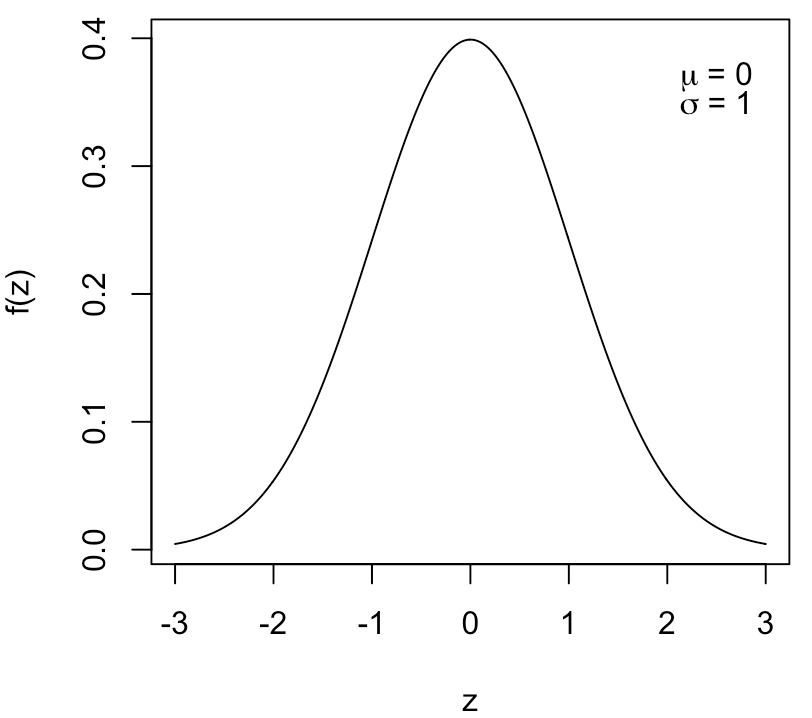
\includegraphics[scale=0.3]{test-3/z}
    \end{figure}
        \item This density function equation looks simpler, but still requires numerical integration.
        \item Forming $(X - \mu) / \sigma$ is known as \textbf{standardizing} $X$. Note that we can standardize any random variable, not just normals.
        \item Example: Suppose $X \follow{Exponential}(\lambda)$.\vspace{50pt}
        \item[] However $Z$ doesn't necessarily have the same distribution of $X$.
    \end{itemize}\bigskip
    \item \textbf{Step 3: Using z-tables}\bigskip
    \begin{itemize}
        \item Tables of areas under the density curve for the distribution of $Z$ have been constructed for use in probability calculations.
        \item The table gives values for the cdf of $Z$, $F_Z(z) = P(Z \le z)$.
        \item Can find any probability we would like using the cdf:
        \item[] $P(Z \le z) = $\vspace{20pt}
        \item[] $P(Z > z) = $\vspace{20pt}
        \item[] $P(z_1 \le Z \le z_2) = $\vspace{40pt}
        \item Examples:\vspace{40pt}
    \end{itemize}\bigskip
    \item \textbf{Step 4: Finding probabilities for any normal $\boldsymbol{X}$}\bigskip
    \begin{itemize}
        \item Once we know how to find probabilities for $Z$, we can use the transformation in step 1 to find probabilities for any normal random variable $X$ with mean $\mu$ and standard deviation $\sigma$ using the identity:
        \[P(x_1 \le X \le x_2) = P\Big(\frac{x_1 - \mu}{\sigma} \le \frac{X - \mu}{\sigma} \le \frac{x_2 - \mu}{\sigma}\Big) = P(z_1 \le Z \le z_2)\]
        \item[] where $\displaystyle z_1 = \frac{x_1 - \mu}{\sigma}$ and $\displaystyle z_2 = \frac{x_2 - \mu}{\sigma}$.
        \item National exam examples: If $X \follow{Normal}(\mu = 500, \sigma = 100)$. Find the following probabilities:
        \item[] $P(X \le 800) = $\vspace{60pt}
        \item[] $P(600 \le X \le 750) = $\vspace{60pt}
    \end{itemize}\bigskip
\end{itemize}\bigskip

Percentiles\bigskip
\begin{itemize}
    \item We can also find percentiles of the standard normal distribution from the table.
    \item Recall for $0 \le p \le 1$ the \textbf{100}$\boldsymbol{p^{th}}$ \textbf{percentile} of $X$ is the number $x_p$ defined by
    \[F(x_p) = p\]
    \item If $X$ is a normal random variable with mean $\mu$ and standard deviation $\sigma$, then we can easily find $x_p$, using $z_p$ and the basic relationship of $X$ and $Z$.
    \[z_p = \frac{x_p - \mu}{\sigma}\]
    \item Examples: If you scored in the $70^{th}$ percentile of test scores, what was your score?\vspace{140pt}
    \item[] Find the test score corresponding to the top 15\% of scores.\vspace{100pt}
    \item This can also be done using software such as TI-84s.
    \begin{figure}[H]
        \center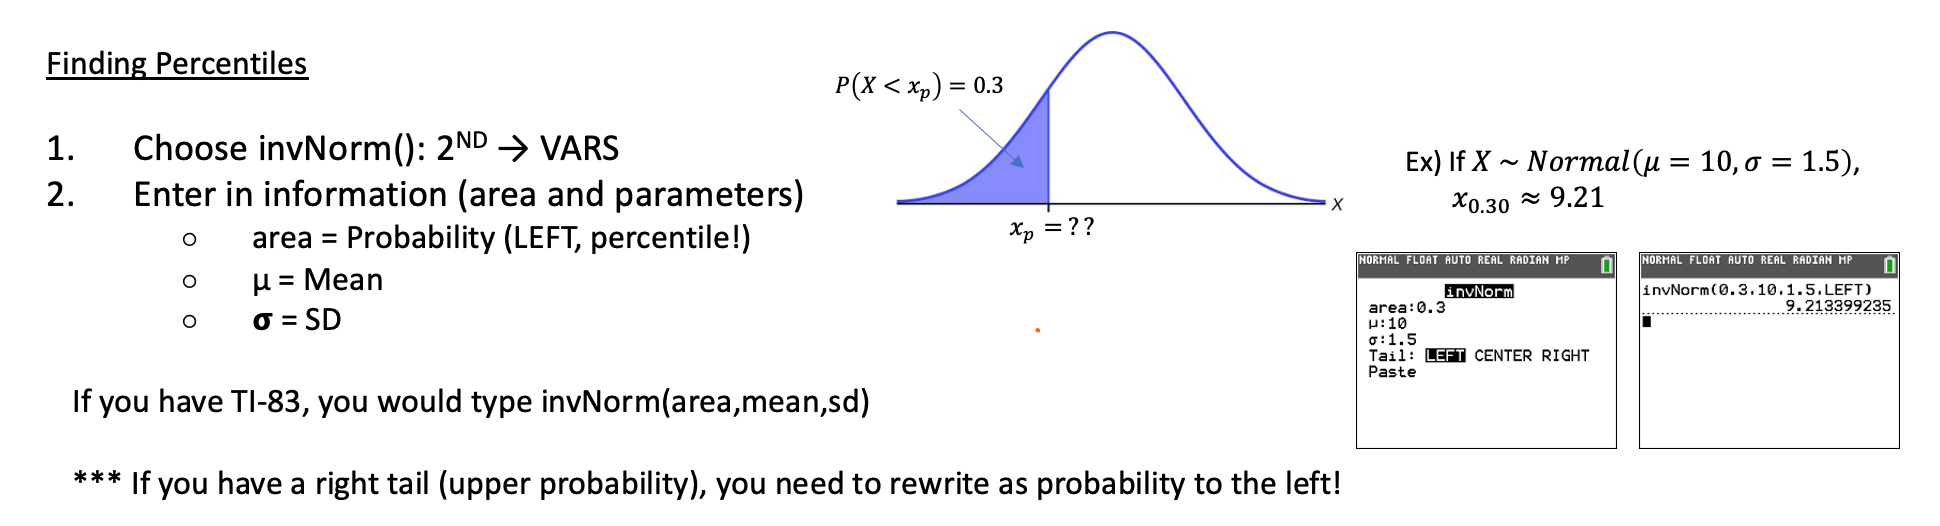
\includegraphics[scale=0.45]{test-3/percentiles}
    \end{figure}
\end{itemize}\bigskip

Harder examples\bigskip
\begin{enumerate}
    \item Let $X \follow{N}(\mu, \sigma^2)$, $P(X < 500) = 0.5$ and $P(X > 650) = 0.0228$.
    \item[] Find $\mu$ and $\sigma^2$.\vspace{130pt}
    \item Let $X \follow{N}(\mu = 25, \sigma^2 = 36)$. Find $c$ such that $P(\lvert X - 25 \rvert \le c) = 0.9544$\vspace{130pt}
    \item If $X \follow{N}(\mu = 1, \sigma^2 = 16)$, find $P(X^2 - 4X < 21)$.\vspace{130pt}
\end{enumerate}\bigskip

\bu{Central Limit Theorem}\bigskip

Sums of independent, identically distribution random variables\bigskip
\begin{itemize}
    \item We will now demonstrate one reason why the normal distribution is so useful in applications.
    \item Motivating example: Recall the previous straight-line density example, where the random variable $X$ represented the loss on a single warranty insurance policy. It was not normally distributed.
    \item[] We found that $E(X) = \frac{100}{3}$ and $V(X) = \frac{5,000}{9 }$ and were able to find probabilities for $X$. However, this information applies only to a single policy.
    \item[] The company selling insurance has more than one policy and must look at its total book of business by adding up all of the losses on all policies.\bigskip
    \item Generalizing this scenario: Suppose the loss on a single insurance policy follows a non-normal density $X$. Companies will have say 1,000 policies and be interested in the total loss $S$, which is the sum of the losses on all individual policies $X_i$:
    \[S = X_1 + X_2 + \cdots + X_{1000}\]
    \item If we assume that all of the policies are $iid$ (independent and follow the same distribution), then the \textbf{Central Limit Theorem (CLT)} shows the sum is approximately normal (even though the individual policies $X_i$ are not) $\Longrightarrow$ which means we can use normal probability methods to find probabilities for the total loss.\bigskip
    \item \textbf{Central Limit Theorem} Let $\vectwo{X}{n}$ be independent random variables, all of which have the same probability distribution and thus the same mean $\mu$ and variance $\sigma^2$. If $n$ is large, the sum
    \[S = X_1 + X_2 + \cdots + X_n\]
    \item[] will be \ul{approximately normal} with mean $n\mu$ and variance $n\sigma^2$.
    \item[] Written succinctly:\vspace{40pt}
    \item Notes about CLT:
    \begin{itemize}
        \item This is a super powerful theorem!
        \item $X_i$ do not have to be normally distributed. When this is the case, the CLT results in an approximately normal distribution.
        \item How large must $n$ be? This depends on how close the original distribution is to the normal.
        \item[] Some elementary statistics books define $n \ge 30$ as ``large''. This will not always be the case. For example, skewed distributions will require larger values of $n$ compared to symmetric distributions in order for the results of the CLT to be decent.
        \item In general, as $n$ increases, approximations based on the CLT get better and better. 
        \item If $X_i \followsp{iid}{Normal}(\mu, \sigma^2)$, then the CLT results in an exactly normal distribution for all $n$.
    \end{itemize}\bigskip
    \item Return to motivating example: Find the distribution of the sum of losses $S$.\vspace{30pt}
    \item[] Find the probability total losses are less than \$35,000.\vspace{70pt}
    \item[] This shows the company that it is not likely to need more than \$35,000 to pay claims, which is helpful in planning.
\end{itemize}\bigskip

More examples\bigskip
\begin{enumerate}
    \item Another example: Suppose the number of claims filed on for a particular policy follow a Poisson distribution with a mean of 2 claims per year and the company has a portfolio of 500 active policies this year, which are assumed to be independent.
    \begin{enumerate}
        \item Find the distribution of the total number of filed claims for the entire portfolio.\vspace{80pt}
        \item Find the probability there will be more 1060 claims this year.\vspace{80pt}
    \end{enumerate}
    \item Two instruments are used to measure the height, $h$, of a tower. The error made by the less accurate instrument is normally distributed with mean 0 and standard deviation $0.0056h$. The error made by the more accurate instrument is normally distributed with mean 0 and standard deviation $0.0044h$. Assuming the two measurements are independent random variables, what is the probability that their average value is within $.005h$ of 0?\vspace{200pt}
\end{enumerate}\bigskip

Summary\bigskip
\begin{itemize}
    \item In general, normal distribution is quite valuable because it applies in so many situations were independent and identical components are being added.
    \item[]Even though normal is continuous, the CLT works with discrete distributions as we saw above.
    \item And the CLT showed us why so many random variables are approximately normally distributed.
    \item[] This occurs because many useful random variables are themselves sums of other independent random variables.
\end{itemize}\bigskip

\newpage

\bu{Lognormal distribution}\bigskip

(Brief) Motivation\bigskip
\begin{itemize}
    \item An alternative to the gamma distribution for asymmetric data is the lognormal distribution.
    \item[] This distribution is more widely used than gamma to model skewed populations because we can take advantage of the properties of the normal distribution.
    \item Examples include insurance claim severity and investment returns.
\end{itemize}\bigskip

Definition\bigskip
\begin{itemize}
    \item A random variable is called \textbf{lognormal} if its natural logarithm is normally distributed.
    \item[] If $Y \follow{Lognormal} \Longleftrightarrow \ln(Y) \follow{Normal}(\mu, \sigma^2)$.\bigskip
    \item Stated another way: A random variable $Y$ is lognormal if $Y = \e^X$ for some normal random variable $X$ with mean $\mu$ and variance $\sigma^2$.
    \item[] If $X \follow{Normal}(\mu, \sigma^2)$ and $Y = \e^X \Longleftrightarrow Y \follow{Lognormal}$
    \[f(y \mid \mu, \sigma^2) = \frac{1}{y \sqrt{2 \pi \sigma^2}} \, \exp\bigg[-\frac{(\ln(y) - \mu)^2}{2\sigma^2}\bigg], \quad\quad  y \ge 0 \quad \text{and}\quad -\infty < \mu < \infty, \quad \sigma > 0\]\vspace{30pt}
    \item Characteristics of a lognormal distribution.
    \begin{itemize}
        \item Right-skewed density function.
        \item Unbounded support.
    \end{itemize}
\end{itemize}\bigskip

Parameters, expected value and variance\bigskip
\begin{itemize}
    \item Note that the parameters $\mu$ and $\sigma^2$ represent the mean and variance of the normal random variable $X$ which appears in the exponent.
    \item Here is how they affect the lognormal density function.
    \begin{figure}[H]
       \begin{minipage}{0.45\textwidth}
            \center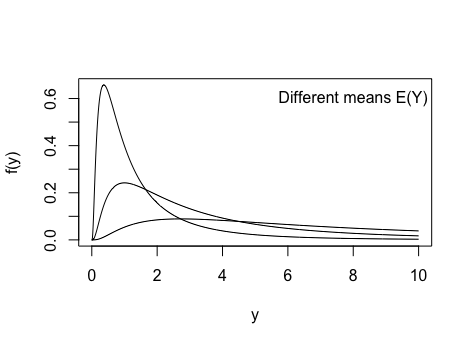
\includegraphics[scale=0.3]{test-3/lognormal-means}
        \end{minipage}
       \begin{minipage}{0.45\textwidth}
            \center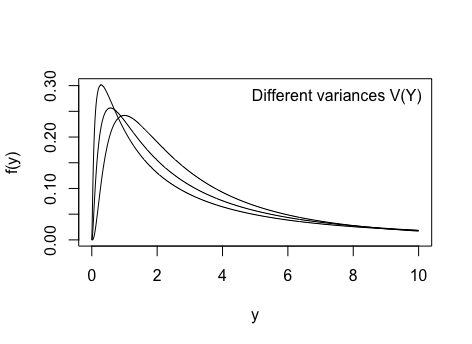
\includegraphics[scale=0.3]{test-3/lognormal-sds}
        \end{minipage}
    \end{figure}
    \item The mean and variance of the actual lognormal distribution $Y$ are:
    \item[] If $X \follow{Normal}(\mu, \sigma^2)$ and $Y = \e^X$
    \[E(Y) = \e^{\mu + \frac{\sigma^2}{2}} \hspace{80pt} V(Y) = \e^{2\mu + \sigma^2} (\e^{\sigma^2} - 1)\]
\end{itemize}\bigskip

Probabilities\bigskip
\begin{itemize}
    \item Just like with the normal, we cannot integrate the pdf, but we do not need to. The cdf can be found directly from the cdf for the normally distributed exponent.
    \item $F_Y(y) = $\bigskip
    \item This means we just need to do algebra in the probability statement, then use \\normalcdf() or $z$-tables like normal on the resulting number.
\end{itemize}\bigskip

Example\bigskip
\begin{itemize}
    \item Let the claim severity $X \follow{Normal}(\mu = 7, \sigma^2 = 49)$ and $Y = \e^X$.
    \begin{enumerate}[(a)]
        \item Find $E(Y)$ and $V(Y)$.\vspace{30pt}
        \item Find the probability a claim is less than or equal to 1300.\vspace{100pt}
        \item Find the probability a claim is between 900 and 1200.\vspace{100pt}
    \end{enumerate}
\end{itemize}

\newpage

\bu{Beta distribution}\bigskip

(Brief) Motivation\bigskip
\begin{itemize}
    \item The beta distribution is defined on the interval $[0, 1]$. 
    \item Thus it is often used as a model for \blankul{4cm} such as the proportion of impurities in a chemical product or the proportion of time that a machine is under repair
\end{itemize}\bigskip

Definition\bigskip
\begin{itemize}
    \item If $X \follow{Beta}(\alpha, \beta)$\bigskip
    \[f(x \mid \alpha, \beta) = \frac{1}{\Beta{\alpha}{\beta}} \, x^{\alpha-1} (1 - x)^{\beta-1}, \quad\quad  0  \le x \le 1 \quad \text{and}\quad \alpha, \beta > 0,\]
    \item[] where
    \[\Beta{\alpha}{\beta} = \integral{0}{1}{x^{\alpha-1} (1 - x)^{\beta-1}}{x} = \frac{\gam{\alpha}\gam{\beta}}{\gam{\alpha + \beta}}\]
    \item Intuitive idea behind pdf: Like the gamma distribution, we construct the formula as the function of $x$ and then find the constant out from to make the density valid.
    \item Characteristics of a beta distribution.
    \begin{itemize}
        \item In general, asymmetric density function.
        \item Bounded support.
    \end{itemize}
\end{itemize}\bigskip

Parameters, expected value and variance\bigskip
\begin{itemize}
    \item The beta random variable $X$ is often used as a model for probability and proportion. Thus, $x$ represents the probability of success and $1 - x$ represents the probability of failure.
    \item[] So, $\alpha$ and $\beta$ sort of represent the chances (or weight) of success and failure, respectively.
    \item For example, when $\alpha = 5$ and $\beta = 2$, the chance of success is stronger than the chance of failure. So the mode and mean lean towards 1. In addition, as the parameters increase, the distributions tighten around the expectations.\bigskip
    \begin{figure}[H]
        \center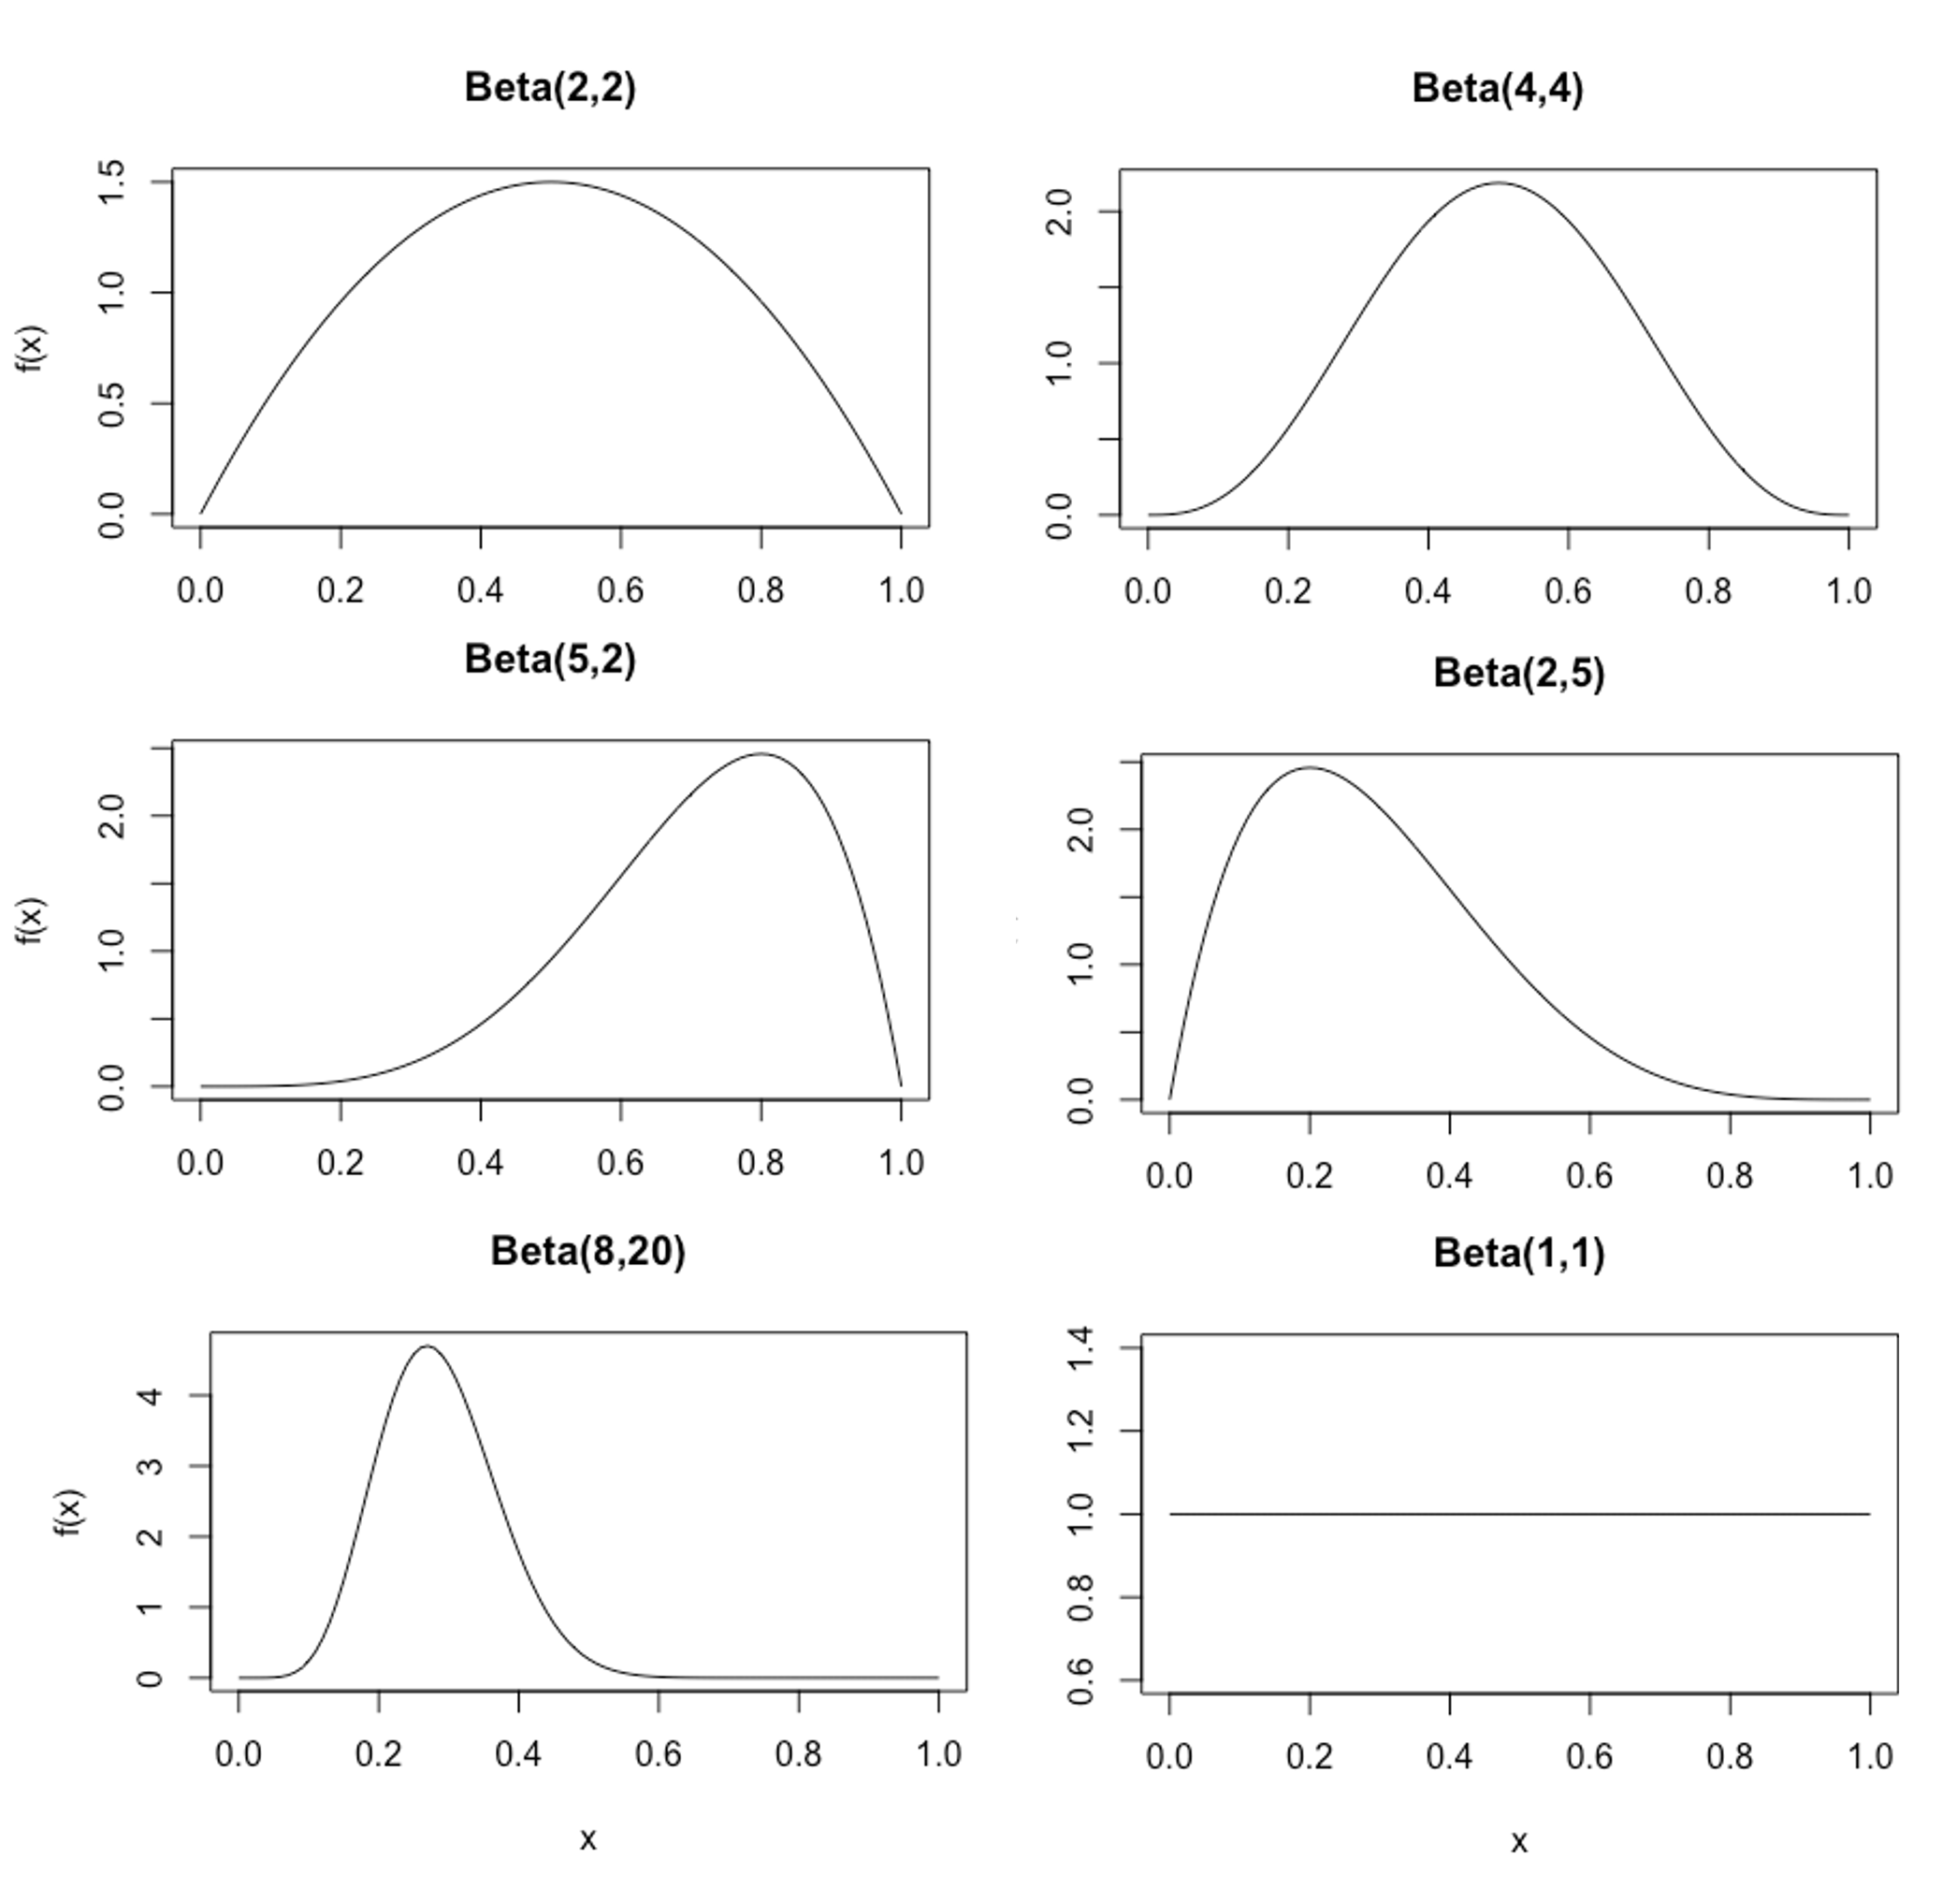
\includegraphics[scale=0.375]{test-3/beta-dists}
    \end{figure}
    \item If $X \follow{Beta}(\alpha, \beta)$
    \[E(X) = \frac{\alpha}{\alpha + \beta} \hspace{80pt} V(X) = \frac{\alpha \beta}{(\alpha + \beta)^2 (\alpha + \beta + 1)}\]
\end{itemize}

Probabilities\bigskip
\begin{itemize}
    \item When $\alpha$ and $\beta$ are integers greater than 1, the cdf can be found by integrating a polynomial. Else we need to use software.
\end{itemize}\bigskip

Example\bigskip
\begin{itemize}
    \item A management firm handles investment accounts for a large number of clients. The percent of clients who contact the firm for information or services in a given month is a beta random variable with $\alpha = 4$ and $\beta = 3$.
    \begin{enumerate}[(a)]
        \item Find the pdf $f(x)$ and the cdf $F(x)$.\vspace{100pt}
        \item Find the probability the percent of clients contacting the firm in a month is less than 40\%.\vspace{20pt}
        \item Find the expected value and variance for the percent of clients contacting the firm.\vspace{20pt}
    \end{enumerate}
\end{itemize}\bigskip

\bu{Transformations}\bigskip

\begin{itemize}
    \item We have covered the standard shapes that can be modeled by these distributions. To be more flexible, we can use functions of these random variables to model variations of the standard shapes.
    \item Examples:
    \begin{enumerate}
        \item If a population is left-skewed and the range is $-\infty < Y \le 0$. How can we model the population?
        \begin{figure}[H]
            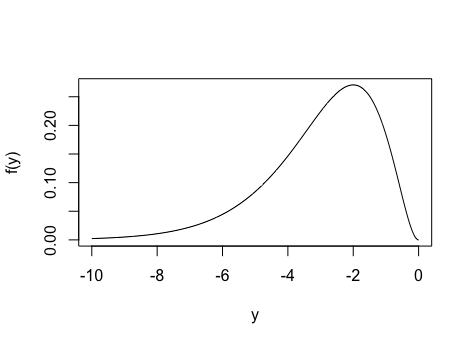
\includegraphics[scale=0.2]{test-3/left-skewed}
        \end{figure}
        \item If a population is right-skewed, but the range is $a \le Y < \infty$, $a \ne 0$. How can we model the population?
        \begin{figure}[H]
            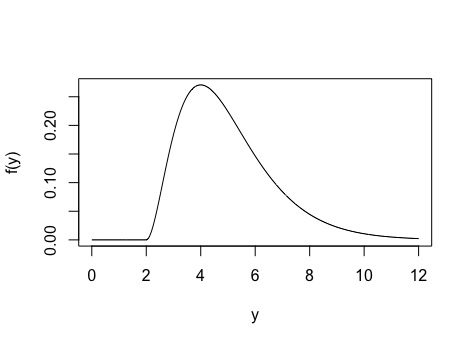
\includegraphics[scale=0.2]{test-3/right-skewed-shift}
        \end{figure}
        \item If a population is left-skewed and the range is $-\infty < Y \le a$, $a \ne 0$. How can we model the population?
        \begin{figure}[H]
            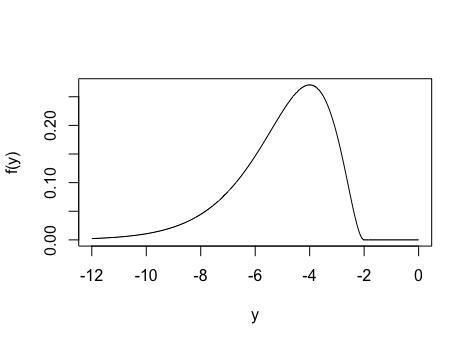
\includegraphics[scale=0.2]{test-3/left-skewed-shift}
        \end{figure}
        \item If a population is bounded between $a \le Y \le b$. How can we model the population?
        \begin{figure}[H]
            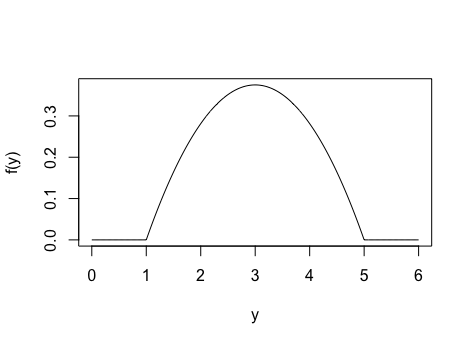
\includegraphics[scale=0.2]{test-3/bounded-range}
        \end{figure}
    \end{enumerate}
\end{itemize}

\end{document}